% Kapittel 3 - Konstruksjon
\chapter{Konstruksjon}
\label{konstruksjon} % Bruk \ref{konstruksjon}, for å referere til kapittelet andre steder i oppgaven. 
%----------------------------------------------------------------------------------------

\todo[inline]{Mats/Tobias: Skrive introduksjon}
%----------------------------------------------------------------------------------------
\begin{comment}
\section{Designmønster brukt i applikasjonen}
\subsection{Arkitekturmodellen Model View Controller}
Model View Controller er en arkitektur som vanligvis blir brukt for å utvikle brukergrensesnitt som deler opp applikasjonen i tre ulike deler. MVC-arkitekturen deler opp store komponenter, slik at en kan bruke samme kode på flere steder \cite{MVC_uses}. Denne arkitekturen har i senere tid blitt svært populær for designing av nett- og mobilapplikasjoner. Populære programmeringsspråk som Java, C\#, Python, Ruby og PHP har MVC-rammeverk som er brukt i webutvikling. 

\subsubsection{Komponentene i Model View Controller}
Slik som med andre designmønster så er MVC kun kjernen av arkitekturen. Det finnes nok mange MVC arkitekturer som kan skille seg fra den generelle forklaringen under, men den gir et godt bilde på grunnprinsippet \cite{MVC_coreArc}.
\begin{itemize}
    \item Modellen (model) er den sentrale komponenten av mønsteret. Det er applikasjonens dynamiske datastruktur, uavhengig av brukergrensesnittet. Det håndterer data, logikk og regler i applikasjonen.
    \item En visning (view) kan være en fremvisning av informasjon. Det er mulig å ha flere visninger for samme informasjon. For eksempel kan visningen være både en tabell og en graf som viser til samme data. 
    \item Kontrolleren (controller) tar brukerinput og konverterer det til kommandoer for enten modellen eller visningen \cite{MVC_components}. 
\end{itemize}

\subsubsection{Relasjonene mellom komponentene i Model View Controller}
I tillegg til å dele applikasjonen inn i tre komponenter, så bestemmer også MVC-designet relasjonene mellom dem. 
\begin{itemize}
    \item Modellen har ansvaret for å håndtere all data i applikasjonen. Den mottar brukerinput fra kontrolleren.
    \item Visningen presenterer modellen i et spesifikt format.
    \item Kontrolleren responderer på brukerinputen og utfører operasjoner på objektene fra datamodellen. Kontrolleren mottar inputen før den eventuelt validerer den og så sender den videre til modellen \cite{MVC_relations}.
\end{itemize}
\begin{figure}[ht]
    \centering
    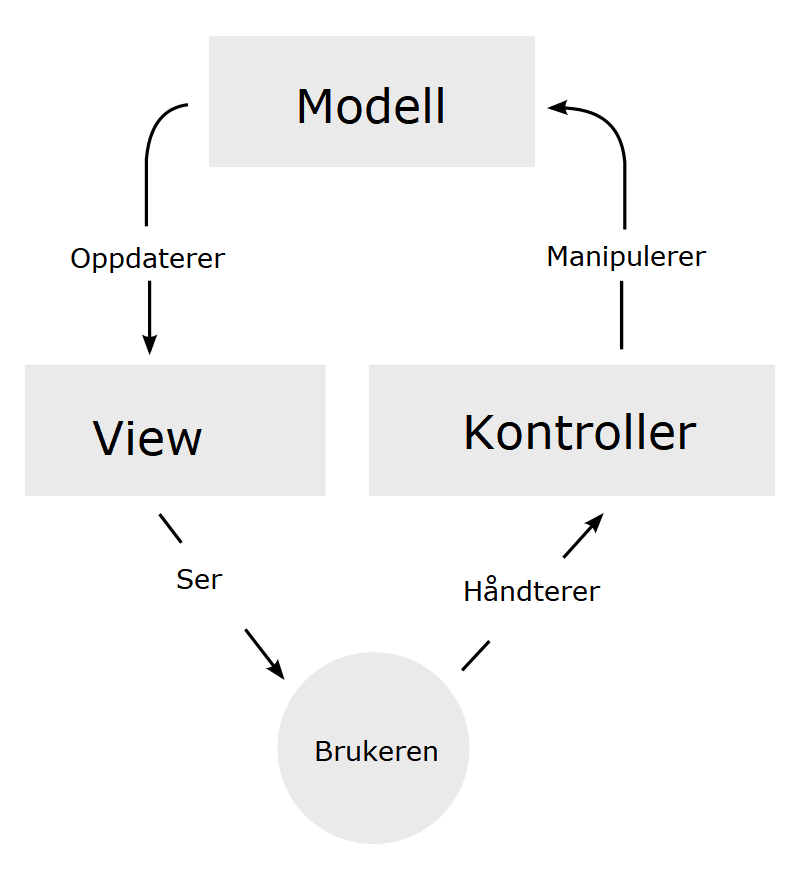
\includegraphics[width=0.7\textwidth]{Figurer/MVC_prosess.png}
    \caption{Relasjoner mellom komponentene i en Model View Controller arkitektur}
    \label{fig:mvc_relations}
\end{figure}

\subsubsection{Fordeler og ulemper med Model View Controller}
Fordeler:
\begin{itemize}
    \item Samarbeid under utvikling: Flere utviklere kan arbeide samtidig på modellen, kontrolleren og visningene. 
    \item Enklere å modifisere: Siden de ulike komponentene har egne ansvarsområder, så er det lettere å gjøre endringer på applikasjonen senere.
    \item Modellen kan ha flere visninger
\end{itemize}
Ulempe:
\begin{itemize}
    \item Omfattende: Rammeverket kan være vanskelig å forstå fordi det introduserer mange nye begrep, sammenhenger og relasjoner som må læres.
\end{itemize}

\subsection{Avhengighetsinjeksjon}% Dependency Injection
\begin{wrapfigure}[16]{r}{0.35\textwidth}
    \centering
    
\includegraphics[width=0.3\textwidth]{Figurer/Dependency_injection.png}
    \caption{Tjeneste brukt i en komponent \cite{angularDI}}
    \label{fig:di}
\end{wrapfigure}

Avhengighetsinjeksjon er et designmønster hvor klasser får avhengigheter fra eksterne kilder, istedenfor å opprette dem selv. Dette gjør at flere klasser kan dele samme ressurs og på den måten øker man modulariteten i applikasjonen \cite{whatIsDI}.

Et typisk eksempel hvor avhengighetsinjeksjon blir brukt i Angular, er tjenester. En tjeneste defineres med en spesifikk funksjon som alle komponentene kan abonnere på hvis de trenger denne (som vist i figur \ref{fig:di}).
\end{comment}
%----------------------------------------------------------------------------------
\section{Designmønster i applikasjonen}
MVC? Mobile first?
\section{Komponentene i applikasjonen}
Man pleier ofte å omtale relasjoner mellom komponenter som om vi snakker om en familie. I applikasjonen er det én rotkomponent. Denne er forelderen til de fire andre komponentene som finnes i applikasjonen. De fire barnekomponentene (navigasjonslinjen, tabellen, innstillingene og grafen i applikasjonen) arver fra forelderen sin (rotkomponenten). Barnekomponentene blir sett på som søsken. Det vil si at de også kan kommunisere med søskena sine, for eksempel ved bruk av tjenester (kapittel \ref{tjenesterRef}) \cite{angularComponents}. 
%\begin{figure}[ht]
%    \centering
%    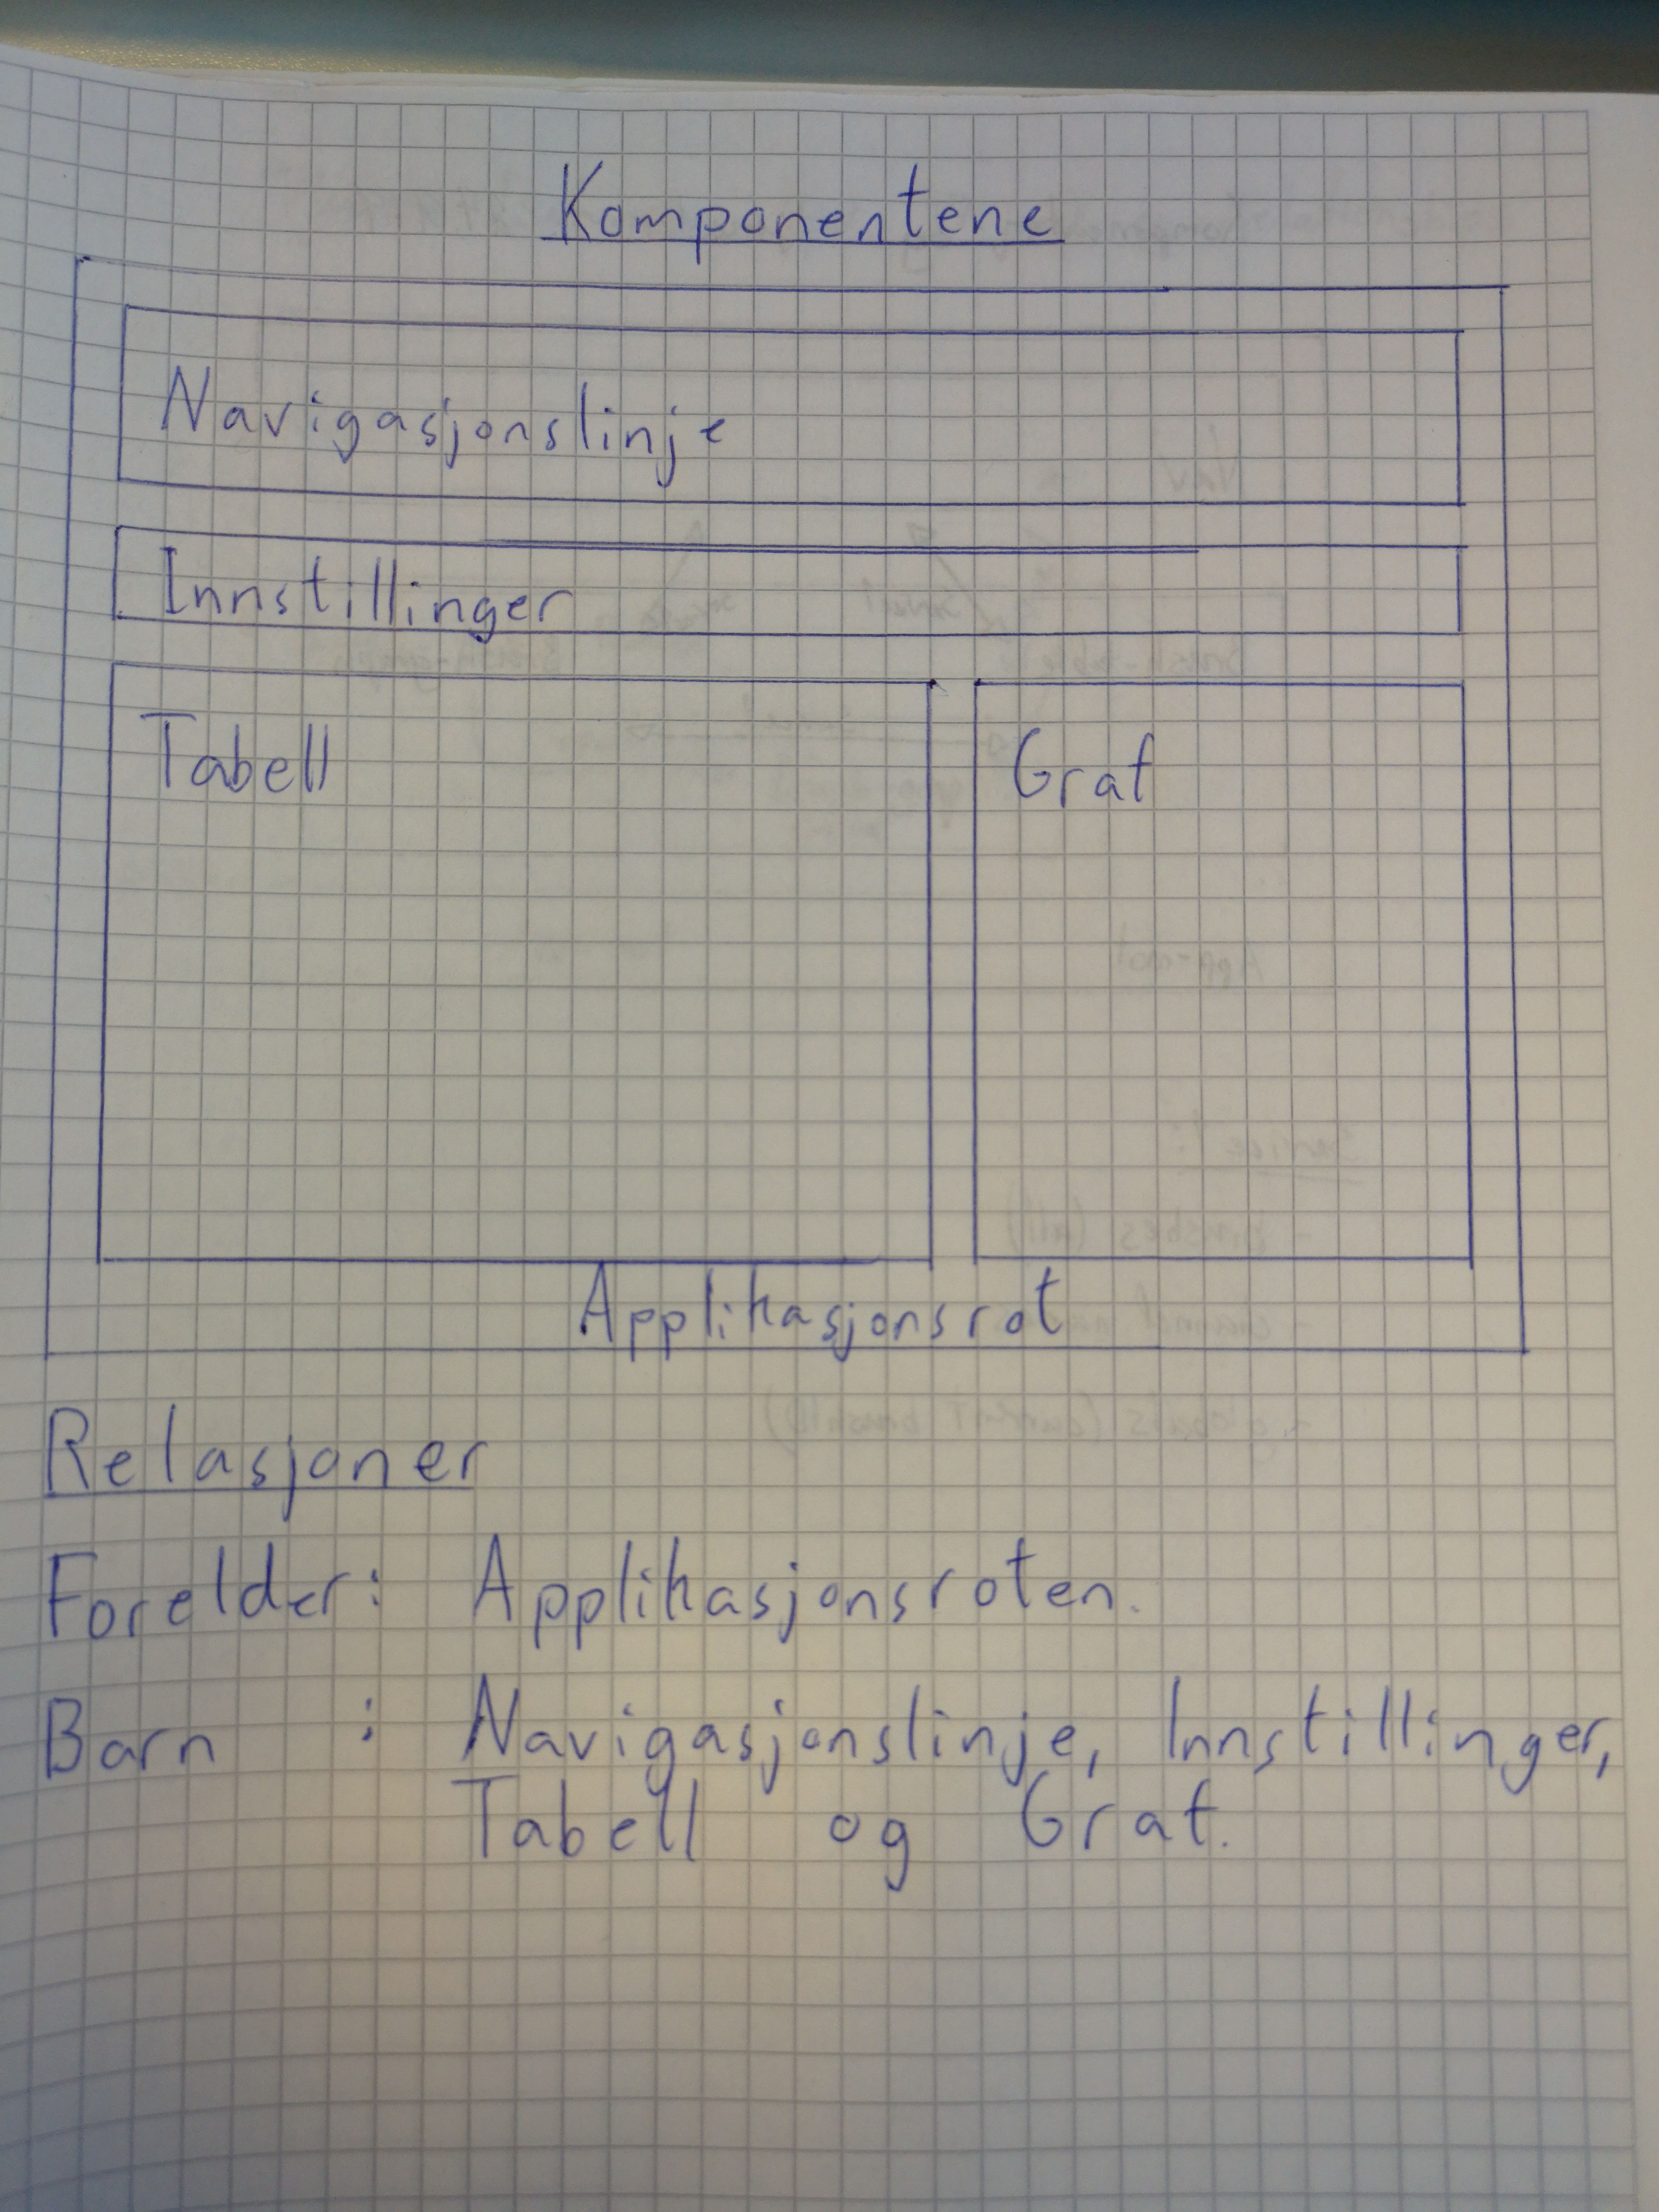
\includegraphics[width=0.6\textwidth]{Figurer/Komponenter_skisse.jpg}
%    \caption{Her vises rotkomponenten med alle barnekomponentene}
%    \label{fig:komponenter_skisse}
%\end{figure}

\subsection{Navigasjonslinjen i applikasjonen}
Den øverste komponenten i applikasjonen er navigasjonslinjen. Her vil man finne alle de viktigste valgene og mulighet for å vise/skjule andre komponenter. Navigasjonslinjen er basert på Bootstrap sin navigasjonsbar og gir et ryddig og oversiktlig utseende. Navigasjonslinjen komprimeres også hvis applikasjonen brukes på enheter med liten skjerm slik at den ikke opptar for mye plass. 

Når man åpner applikasjonen først gang, får man to valg i navigasjonslinjen; Åpne lokal fil eller åpne fil lokalisert på roboten. Når en fil er åpnet, dukker det opp flere valg i menyen. Man kan da velge å eksportere filen (både lokalt og til robot), slik at man kan ta vare på eventuelle endringer man har gjort. I tillegg synliggjøres to knapper som gjør det mulig å vise/skjule innstillinger og filinformasjon.

\subsection{Innstillinger i applikasjonen}
Applikasjonen inkludere en komponent for å sette ulike innstillinger. Denne komponenten inneholder alle innstillinger som ikke er knyttet til filinformasjon eller åpning/eksportering av fil. Komponenten vises ved hjelp av valget i navigasjonslinjen og skjules igjen ved hjelp av valget i navigasjonslinjen eller «X»-knappen.

Innstillingene inkludere en knapp for å tilbakestille kanalnavnene til sine standardnavn («Channel 1», «Channel 2» etc.).

\subsection{Filinformasjonskomponenten i applikasjonen}
Denne komponenten viser informasjon knyttet til filen som er lastet inn. Filnavn og eventuelt fil-kommentar vil vises her. Akkurat som innstillingskomponenten vises også denne ved hjelp av valg i navigasjonslinjen og skjules igjen enten ved hjelp av valget i navigasjonslinjen eller «X»-knappen.

\subsection{Informasjonskomponenten i applikasjonen}
For å kunne vise frem informasjon- og feilmeldinger til brukeren, inneholder applikasjonen en informasjonskomponent. Man kan her vise frem tilbakemeldinger til brukeren etter at han/hun har utført en handling. Ett eksempel kan være at man endrer innstillingene. Da kan det vær greit å få en tilbakemelding på om endringene har vært vellykket eller ikke. Dette vil vises i denne komponenten, enten som en vellykket melding eller en feilmelding hvis det har skjedd noe galt. Ved en feilmelding vil man også vise hva som har er galt, slik at man forhåpentligvis kan rette dette opp.

\subsection{Tabellen i applikasjonen}
\todo[inline]{Tobias skriv her}
Tabellen inneholder informasjon om børsten som er lastet inn. Den kan inneholde mellom tre og fem kolonner avhengig av hvor mange ulike kanaler man har i filen. Etter innholdet er lastet inn vil det være mulig å endre på innholdet ved hjelp av dynamiske inputfelt. Grafen blir oppdatert deretter. Hvert felt har en egen maksimumsverdi. 

%\begin{figure}[ht]
%    \centering
%    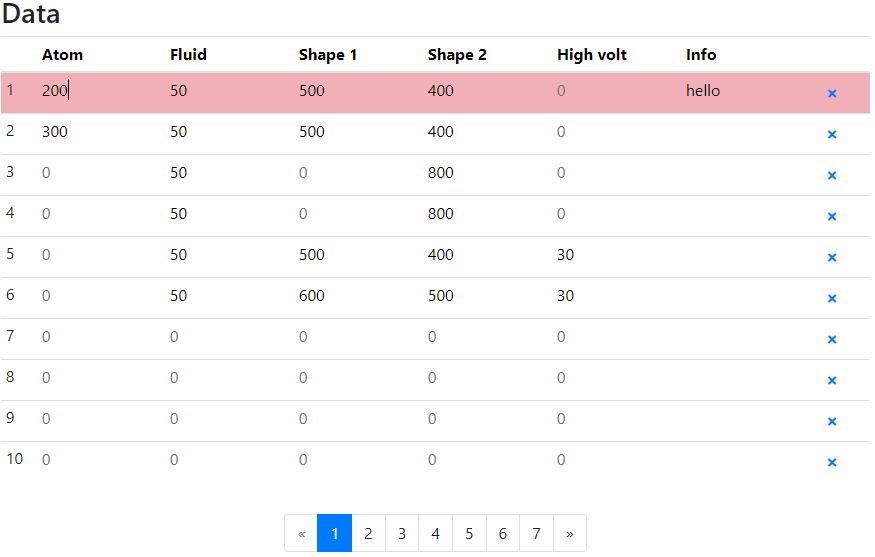
\includegraphics[width=\textwidth]{Figurer/Applikasjon_tabell.PNG}
%    \caption{Tabellen i applikasjonen}
%    \label{fig:applikasjon_tabell}
%\end{figure}

\subsection{Grafen i applikasjonen}
\todo[inline]{Tobias skriv her}
Grafen viser frem data fra en markert rad i tabellen. Den vil fremvise dataen for hvert markerte felt som et prosenttall av maksimum kapasitet. 

%\begin{figure}[ht]
%    \centering
%    \includegraphics[width=\textwidth]{Figurer/Applikasjon_graf}
%    \caption{Grafen i applikasjonen}
%    \label{fig:applikasjon_graf}
%\end{figure}

\section{Tjenester brukt i applikasjonen}
\label{tjenesterRef}
I Brush Editor-applikasjonen er to tjenester definert; «Brush service» og «Pager service».
\subsection{Brush-tjenesten i applikasjonen}
«Brush-service» blir brukt til å lagre dataene som blir lest inn fra en brush-fil eller hentet fra roboten. Flere av komponentene trenger disse dataene (blant annet tabellen og grafen). Tjenesten gjør det enkelt å dele dataene mellom komponenter som trenger dem. I tillegg blir tjenesten mer robust; det er enkelt å legge til eller fjerne komponenter som bruker brush-dataene uten å gjøre store endringer i applikasjonen.

\subsection{Sideskifter-tjenesten i applikasjonen}
«Pager-service» er en mer funksjonell tjeneste. Denne består av logikken til tabellen sin sideskifter. Ved å inkludere en sideskifter i tabellen, får man en mer oversiktlig tabell hvis man har mange rader med data (noe brush-filene ofte har). Selv om denne tjenesten kun blir brukt i tabell-komponenten var det likevel fordelaktig å splitte denne til en egen tjeneste. Man får da fjernet en del linjer med kode fra tabell-komponenten, samt muligheten til å bruke denne tjenesten andre steder i applikasjonene hvis man trenger det.

\section{Oppsummering av kapittelet}